%%
%% This is file `sample-sigconf.tex',
%% generated with the docstrip utility.
%%
%% The original source files were:
%%
%% samples.dtx  (with options: `sigconf')
%% 
%% IMPORTANT NOTICE:
%% 
%% For the copyright see the source file.
%% 
%% Any modified versions of this file must be renamed
%% with new filenames distinct from sample-sigconf.tex.
%% 
%% For distribution of the original source see the terms
%% for copying and modification in the file samples.dtx.
%% 
%% This generated file may be distributed as long as the
%% original source files, as listed above, are part of the
%% same distribution. (The sources need not necessarily be
%% in the same archive or directory.)
%%
%% Commands for TeXCount
%TC:macro \cite [option:text,text]
%TC:macro \citep [option:text,text]
%TC:macro \citet [option:text,text]
%TC:envir table 0 1
%TC:envir table* 0 1
%TC:envir tabular [ignore] word
%TC:envir displaymath 0 word
%TC:envir math 0 word
%TC:envir comment 0 0
%%
%%
%% The first command in your LaTeX source must be the \documentclass command.
\PassOptionsToPackage{table,xcdraw}{xcolor}
\documentclass[sigconf, nonacm]{acmart}
%% NOTE that a single column version may be required for 
%% submission and peer review. This can be done by changing
%% the \doucmentclass[...]{acmart} in this template to 
%% \documentclass[manuscript,screen]{acmart}
%% 
%% To ensure 100% compatibility, please check the white list of
%% approved LaTeX packages to be used with the Master Article Template at
%% https://www.acm.org/publications/taps/whitelist-of-latex-packages 
%% before creating your document. The white list page provides 
%% information on how to submit additional LaTeX packages for 
%% review and adoption.
%% Fonts used in the template cannot be substituted; margin 
%% adjustments are not allowed.
%%
%%
%% \BibTeX command to typeset BibTeX logo in the docs
\AtBeginDocument{%
  \providecommand\BibTeX{{%
    \normalfont B\kern-0.5em{\scshape i\kern-0.25em b}\kern-0.8em\TeX}}}

%% Rights management information.  This information is sent to you
%% when you complete the rights form.  These commands have SAMPLE
%% values in them; it is your responsibility as an author to replace
%% the commands and values with those provided to you when you
%% complete the rights form.
\setcopyright{none}
\copyrightyear{2022}
\acmYear{2022}
\acmDOI{XXXXXXX.XXXXXXX} 

%% These commands are for a PROCEEDINGS abstract or paper.
\acmConference[Conference acronym 'XX]{Make sure to enter the correct
  conference title from your rights confirmation emai}{June 03--05,
  2018}{Woodstock, NY}
%
%  Uncomment \acmBooktitle if th title of the proceedings is different
%  from ``Proceedings of ...''!
%
%\acmBooktitle{Woodstock '18: ACM Symposium on Neural Gaze Detection,
%  June 03--05, 2018, Woodstock, NY} 
\acmPrice{15.00}
\acmISBN{978-1-4503-XXXX-X/18/06}


%%
%% Submission ID.
%% Use this when submitting an article to a sponsored event. You'll
%% receive a unique submission ID from the organizers
%% of the event, and this ID should be used as the parameter to this command.
%%\acmSubmissionID{123-A56-BU3}

%%
%% For managing citations, it is recommended to use bibliography
%% files in BibTeX format.
%%
%% You can then either use BibTeX with the ACM-Reference-Format style,
%% or BibLaTeX with the acmnumeric or acmauthoryear sytles, that include
%% support for advanced citation of software artefact from the
%% biblatex-software package, also separately available on CTAN.
%%
%% Look at the sample-*-biblatex.tex files for templates showcasing
%% the biblatex styles.
%%

%%
%% The majority of ACM publications use numbered citations and
%% references.  The command \citestyle{authoryear} switches to the
%% "author year" style.
%%
%% If you are preparing content for an event
%% sponsored by ACM SIGGRAPH, you must use the "author year" style of
%% citations and references.
%% Uncommenting
%% the next command will enable that style.
%%\citestyle{acmauthoryear}

%%
%% end of the preamble, start of the body of the document source.

%% Removing ACM Reference Format
\settopmatter{printacmref=false}
\definecolor{darkgreen}{rgb}{0.0, 0.5, 0.0}
\definecolor{darkblue}{rgb}{0.0, 0.0, 1.0}
\newcommand{\RGGB}{$
~^{\text{\color{red}R}}_{\text{\color{darkgreen}G}}
~^{\text{\color{darkgreen}G}}_{\text{\color{darkblue}B}}
$}
\newcommand{\BGGR}{$
~^{\text{\color{darkblue}B}}_{\text{\color{darkgreen}G}}
~^{\text{\color{darkgreen}G}}_{\text{\color{red}R}}
$}
\newcommand{\GRBG}{$
~^{\text{\color{darkgreen}G}}_{\text{\color{darkblue}B}}
~^{\text{\color{red}R}}_{\text{\color{darkgreen}G}}
$}
\newcommand{\GBRG}{$
~^{\text{\color{darkgreen}G}}_{\text{\color{red}R}}
~^{\text{\color{darkblue}B}}_{\text{\color{darkgreen}G}}
$}
\begin{document}

%%
%% The "title" command has an optional parameter,
%% allowing the author to define a "short title" to be used in page headers.
\title{Towards a reliable detection of forgeries based on demosaicing}

%%
%% The "author" command and its associated commands are used to define
%% the authors and their affiliations.
%% Of note is the shared affiliation of the first two authors, and the
%% "authornote" and "authornotemark" commands
%% used to denote shared contribution to the research.
\author{Jérémie Dentan}
\email{jeremie.dentan@polytechnique.org}
\affiliation{%
  \institution{École Polytechnique}
  \country{France}
}

%%
%% By default, the full list of authors will be used in the page
%% headers. Often, this list is too long, and will overlap
%% other information printed in the page headers. This command allows
%% the author to define a more concise list
%% of authors' names for this purpose.
\renewcommand{\shortauthors}{Dentan}

%%
%% The abstract is a short summary of the work to be presented in the
%% article.
\begin{abstract}
This is a review of the paper "Demosaicing to Detect Demosaicing and Image Forgeries" written by Quentin Bammey, Rafael Grompone von Gioi, and Jean-Michel Morel \cite{bammey_demosaicing_2022}, which proposes a demosaicing-based forgery detection method.

More than the general performance of the method proposed by the author, our review mainly focus on the reliability of the detection performed, especially in terms of false detections. Thus, our main objective has been to verify that the assumptions made by on the a-contrario model are valid and lead to reliable detections, quantified by a robust Number of False Alarms (NFA).

The results of our experiments show that despite its good performances in the absence of compression, this forgery detection method leads to an abnormally high number of false alarms compared to the theoretical guarantees of the a-contrario model, when the images are compressed. This proves that the assumptions of this model are not verified. Admittedly, we used a smaller number of demosaicing algorithms for our experiments, and older algorithms. However, at no point does the paper discuss either the assumptions made about these algorithms, or their impact on the reliability of the detection.

Thus, our study shows the importance of empirical or theoretical validation of the set of demosaicing algorithms used for forgery detection, a necessary condition to obtain reliable and industrially usable detections. In particular, we show that the set of algorithms used must (1) present similar performances for any level of image compression and (2) present similar performances for any type of textures on natural images.

\end{abstract}

%%
%% Keywords. The author(s) should pick words that accurately describe
%% the work being presented. Separate the keywords with commas.
\keywords{Demosaicing, Forgery Detection, A-contrario model, Number of False Alarm (NFA)}

%% A "teaser" image appears between the author and affiliation
%% information and the body of the document, and typically spans the
%% page.
\begin{teaserfigure}
  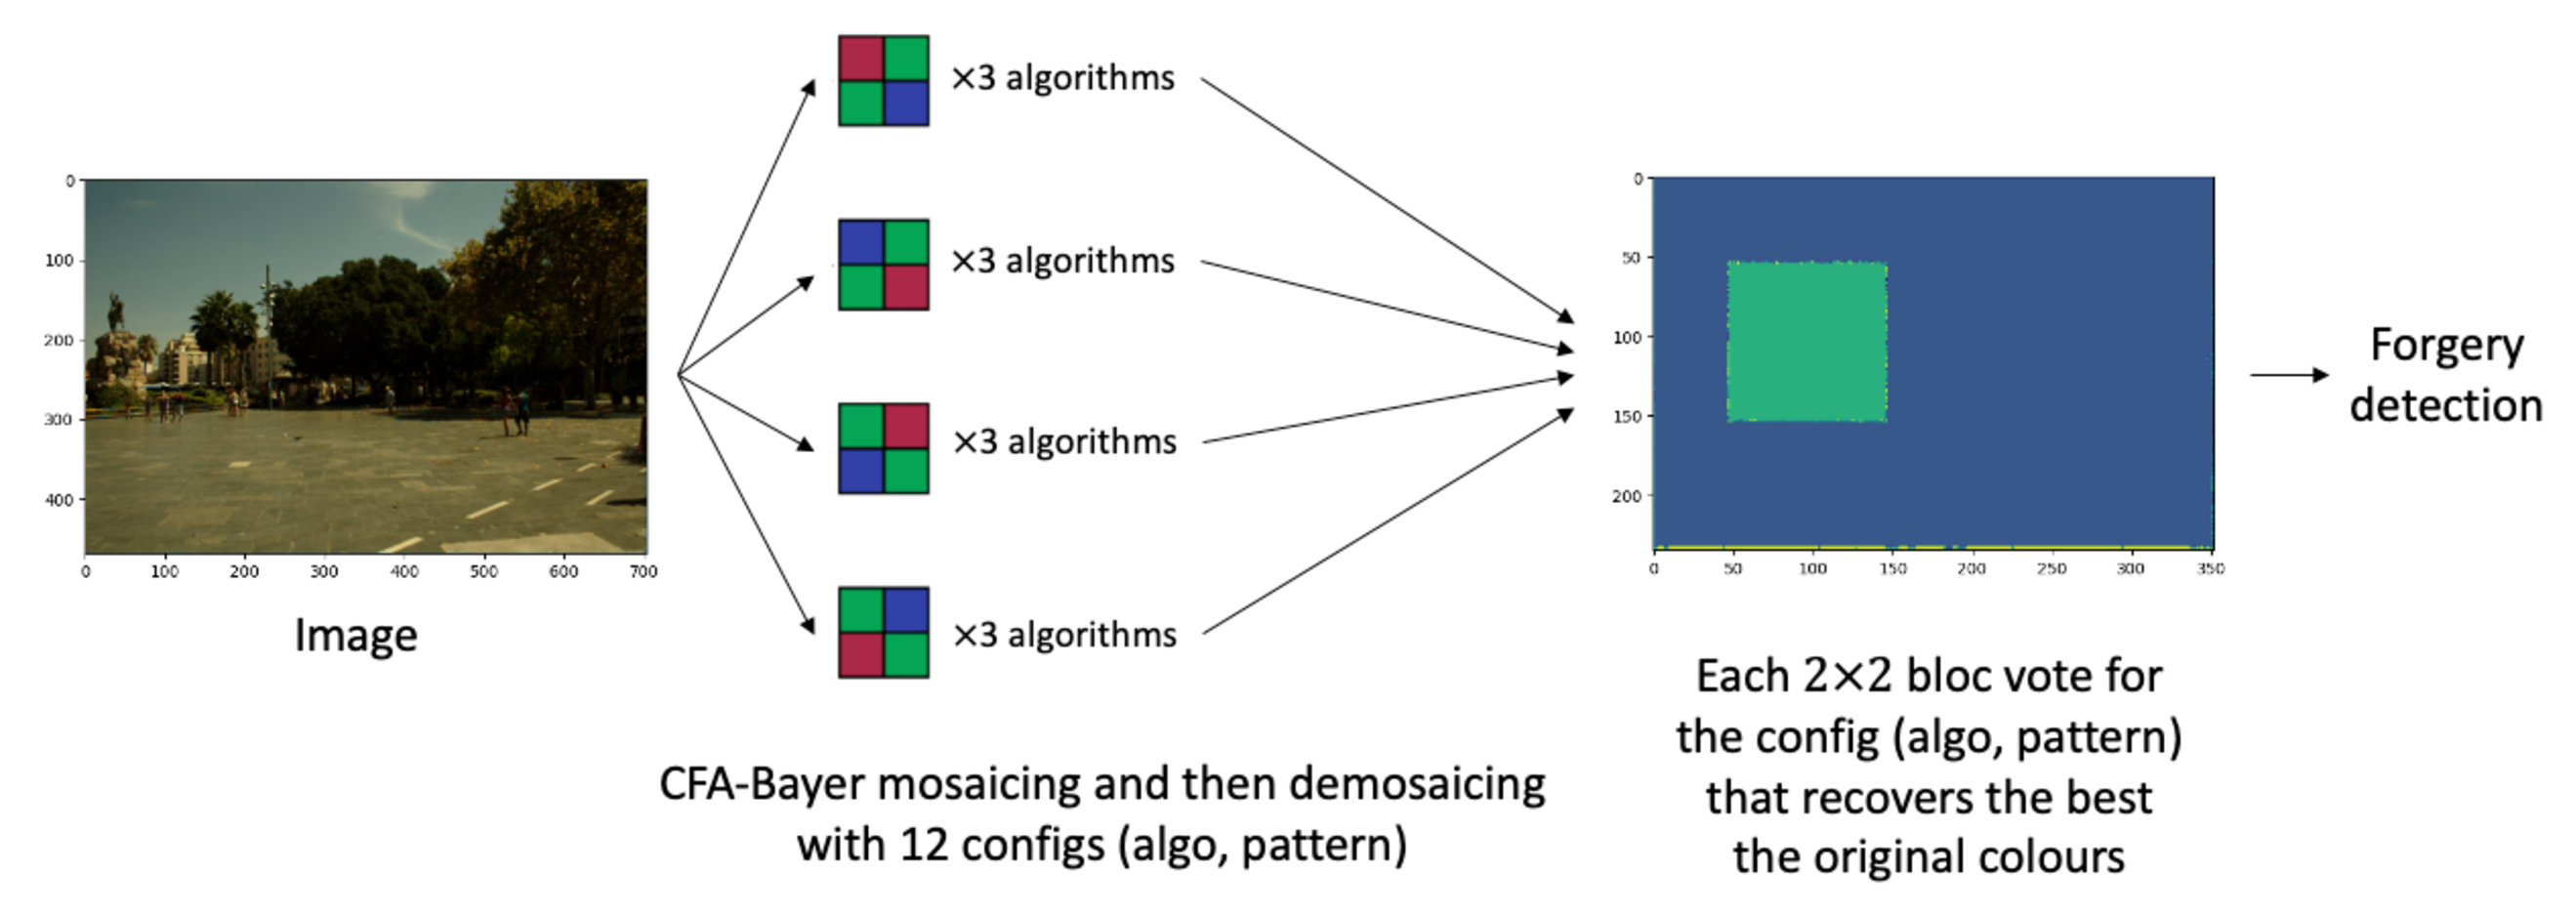
\includegraphics[width=\textwidth]{teaser}
  \caption{General overview of the forgery detection pipeline. {\normalfont The method is based on double demosaicing: an image to be tested is demosaiced using several algorithms and patterns; if several areas of the image are better reconstructed with two different configurations, we can then deduce that one of these areas has been faked.}}
  \label{fig:teaser}
\end{teaserfigure}

\received{01 January 2023}
%\received[revised]{12 March 2009}
%\received[accepted]{5 June 2009}

%%
%% This command processes the author and affiliation and title
%% information and builds the first part of the formatted document.
\maketitle

\section{Introduction} \label{sec:introduction}

This technical report comes with several resources:

\begin{itemize}
    \item A GitHub repository that implements all the experiments made for this review, available \href{https://github.com/DentanJeremie/demosaicing-detection}{\underline{here}}
    \item Two datasets: one provided by \cite{colom_noise_2023}  available \href{http://mcolom.info/pages/no_noise_images/}{\underline{here}}; one provided by the author of this review \cite{dentan_dataset_2023} and available \href{https://gist.github.com/DentanJeremie/21bfd925c5234afd15d854135b569bec}{\underline{here}}
    \item Two notebooks that simply illustrate the methods and assumptions made by this review, and can be run independently, available \href{https://github.com/DentanJeremie/demosaicing-detection/blob/main/doc/forgery_detection_demonstration.ipynb}{\underline{here}} and \href{https://github.com/DentanJeremie/demosaicing-detection/blob/main/doc/configuration_detection_demonstration.ipynb}{\underline{here}}
\end{itemize}

\subsection{Context}

The trustworthiness of images is a significant issue, as digital images can now be easily and convincingly altered using editing tools, making it difficult to assume their accuracy. This creates a pressing need for image analysis in various fields, such as police investigations, fact-checking, and journalism, to detect forgeries. The solution proposed by the authors involves analyzing the traces left by the camera during demosaicing, an initial stage of image formation. Disruption of these traces when an object is added or displaced on an image can leave behind forgery clues.

Most modern cameras cannot detect colors directly, which is why they have a Colour Filter Array (CFA) in front of their sensor. Thus, each pixel perceives only the color corresponding to its filter, and the other colors are interpolated from the values of the neighboring pixels. The Bayer CFA filter is the most widely used nowadays, and that's why it focuses all the attention of the demosaicing detection research. 

For this paper review, we will adopt the following definitions:
\begin{itemize}
    \item \textbf{Mosaicing:} The action of applying a Bayer CFA to an existing image. This steps tries to reproduce a mosaiced image as it would be right after the sensors of a camera. Depending on the offset of the CFA, the mosaicing can be done in one of the four patterns (cf. below).
    \item \textbf{Demosaicing:} Given a mosaiced image, interpolate the RGB colour values of every pixels using the values of the neighboring pixels. The pattern used for the demosaicing should be the same as the one used for the mosaicing.
    \item \textbf{Demosaicing algorithm:} An algorithm that performs demosaicing. For this paper review, we will use the three demosaicing algorithms that are available in the Python \texttt{colour-demosaicing} library: \texttt{bilinear}: simple bilinear interpolation; \texttt{malvar}: an algorithm proposed by Malvar et al. in 2004 \cite{malvar_high-quality_2004}; \texttt{menon}: an algorithm proposed by Menon et al. in 2007 \cite{menon_demosaicing_2007}.
    \item \textbf{Pattern:} one of the four following offset of the CFA: \RGGB, \BGGR, \GBRG, \GRBG.
    \item \textbf{Configuration:} A tuple (demosaicing algorithm, pattern). With our settings, there are 12 of them.
    \item \textbf{Diagonal:} The orientation of the green diagonal in a pattern: 'up' for \RGGB and \BGGR, and 'down' for \GBRG and \GRBG. Indeed, sometimes the diagonal is easier to detect than the precise pattern.
    \item \textbf{Forge:} The action of enforcing the demosaicing configuration of an image. This is done by a mosaicing step immediately followed by a demosaicing step, using the pattern and the demosaicing algorithm we want to enforce. An optional JPEG compression can be done after the forging.
    \item \textbf{Fake:} The action of adding a distortion in the demosaicing of an image (forged or not). This is done by selecting an area in the image, and forging it with a configuration (that is different from the one of the full image, if it has one).
\end{itemize}

\subsection{The method of the article} \label{sec:article_method}

The article describes a method for detecting the demosaicing artefacts in an image. More precisely, there are two types of detections that are discussed in the article, and the different sections of this review discuss separately those detections, even though they are interconnected:

\begin{itemize}
    \item The detection of the demosaicing configuration that was used during the caption of an image. The a-contrario model for this is discussed in section \ref{sec:global_a_contrario}, and we evaluate this detection with the experiment described in section \ref{sec:experiment_1}.
    \item The detection of a region in the image that have different demosaicing artefacts than the other, suggesting that the image is fake. The a-contrario model for this is discussed in section \ref{sec:local_a_contrario}, and we evaluate this detection with the experiment described in section \ref{sec:experiment_2}.
\end{itemize}

The principle of the method proposed by the article, and described in figure \ref{fig:teaser}, is the following:

\begin{itemize}
    \item We have as input an image, and we want to detect if some areas of the image are fake
    \item For the 12 different configuration, we forge the image, resulting in 12 different images of the same shape as the original one
    \item We divide the pixels of the original image in blocks of shape $2 \times 2$. Each block 'votes' for the configuration that approximates it the best, i.e. for the forged image for which the mean absolute difference between the four pixels (the reconstruction error) is the lowest. The idea behind this is that the reconstruction error should be the lowest for the true configuration, i.e. the one that was really used during the caption of the image.
    \item In case of equality, the block votes randomly for one of the configuration that achieves the minimum reconstruction error.
    \item Then, we decide that the image is fake if there is a region in the image that have a lot of votes that are different from what we observe elsewhere in the image (cf. section \ref{sec:a_contrario} for more details). The idea behind this is that for a real natural image, the majority of votes should vote for the real configuration that was used during the caption of the image, so there should be no region where the vote are significantly different. On the opposite, if a piece of image is inserted or displaced, it is likely to have either different pattern of a different demosaicing algorithm.
\end{itemize}

\subsection{Existing literature}

For a more complete overview of the existing literature, we invite you to directly refer to the original paper \cite{bammey_demosaicing_2022}.

Some early work have been done to detect, given an image, the pixel whose colours are interpolated, using either the periodicity of the CFA grid or the variance of the pixel values where the interpolation is done \cite{popescu_exposing_2005, ferrara_image_2012}. Then an important paper have been published in 2010 \cite{memon_detection_2010}, whose work is extended by the paper \cite{bammey_demosaicing_2022} we are reviewing. This paper used a double demosaicing with the four CFA patterns to detect which one have been used for the image. However, this paper only uses bilinear demosaicing, contrary to \cite{bammey_demosaicing_2022}. Then, \cite{milani_demosaicing_2014} applied several demosaicing algorithms using a pattern already detected to detect which one was originally used.

One of the greatest difficulties faced by these different methods is the robustness to compression and in particular JPEG compression \cite{skodras_jpeg_2001}, which is still extremely used today. As explained in the article we are reviewing, very few forgery detection methods based on demosaicing are robust to compression. According to the benchmark proposed in the article, only the 4Point method \cite{bammey_forgery_2022} is robust to compression. It is a method proposed the same year by the same authors, which uses a simple neural network to learn the pattern used during the demosaicing of an image. This method, which is very efficient (according to the same benchmark, it obtains the best performance in all categories), is however very long to execute (about 100 times longer than the approach discussed in this review). This is the reason why it is interesting to explore other numerical methods, lighter, whose performances and robustness, although inferior, are close to those of the 4Point method.

\subsection{Scope of this review}

As said previously, our review mainly focus on the
reliability of the detection performed, especially in terms of false detections. Thus, we will not analyze in detail the benchmark comparing the performance of this method with other state-of-the-art methods. Thus, the main issues we will address in this review concern the automatic detection of fake images using the a contrario framework:

\begin{itemize}
    \item What are the assumptions behind the a contrario model, and are they verified?
    \item Does the number of false alarms (NFA) stated in the article really give confidence in the detection results?
    \item What are the cases where the method fails, and those where it remains effective?
\end{itemize}

\section{The a contrario framework} \label{sec:a_contrario}

\subsection{Introduction}

In this section, we will present the a contrario model used by the paper for detecting image forgery. Our discussion will be based on the definition of \textit{a contrario detection} and \textit{number of false alarm} as presented in \cite{morel_detection_2021}.

\begin{figure}[!h]
    \centering
    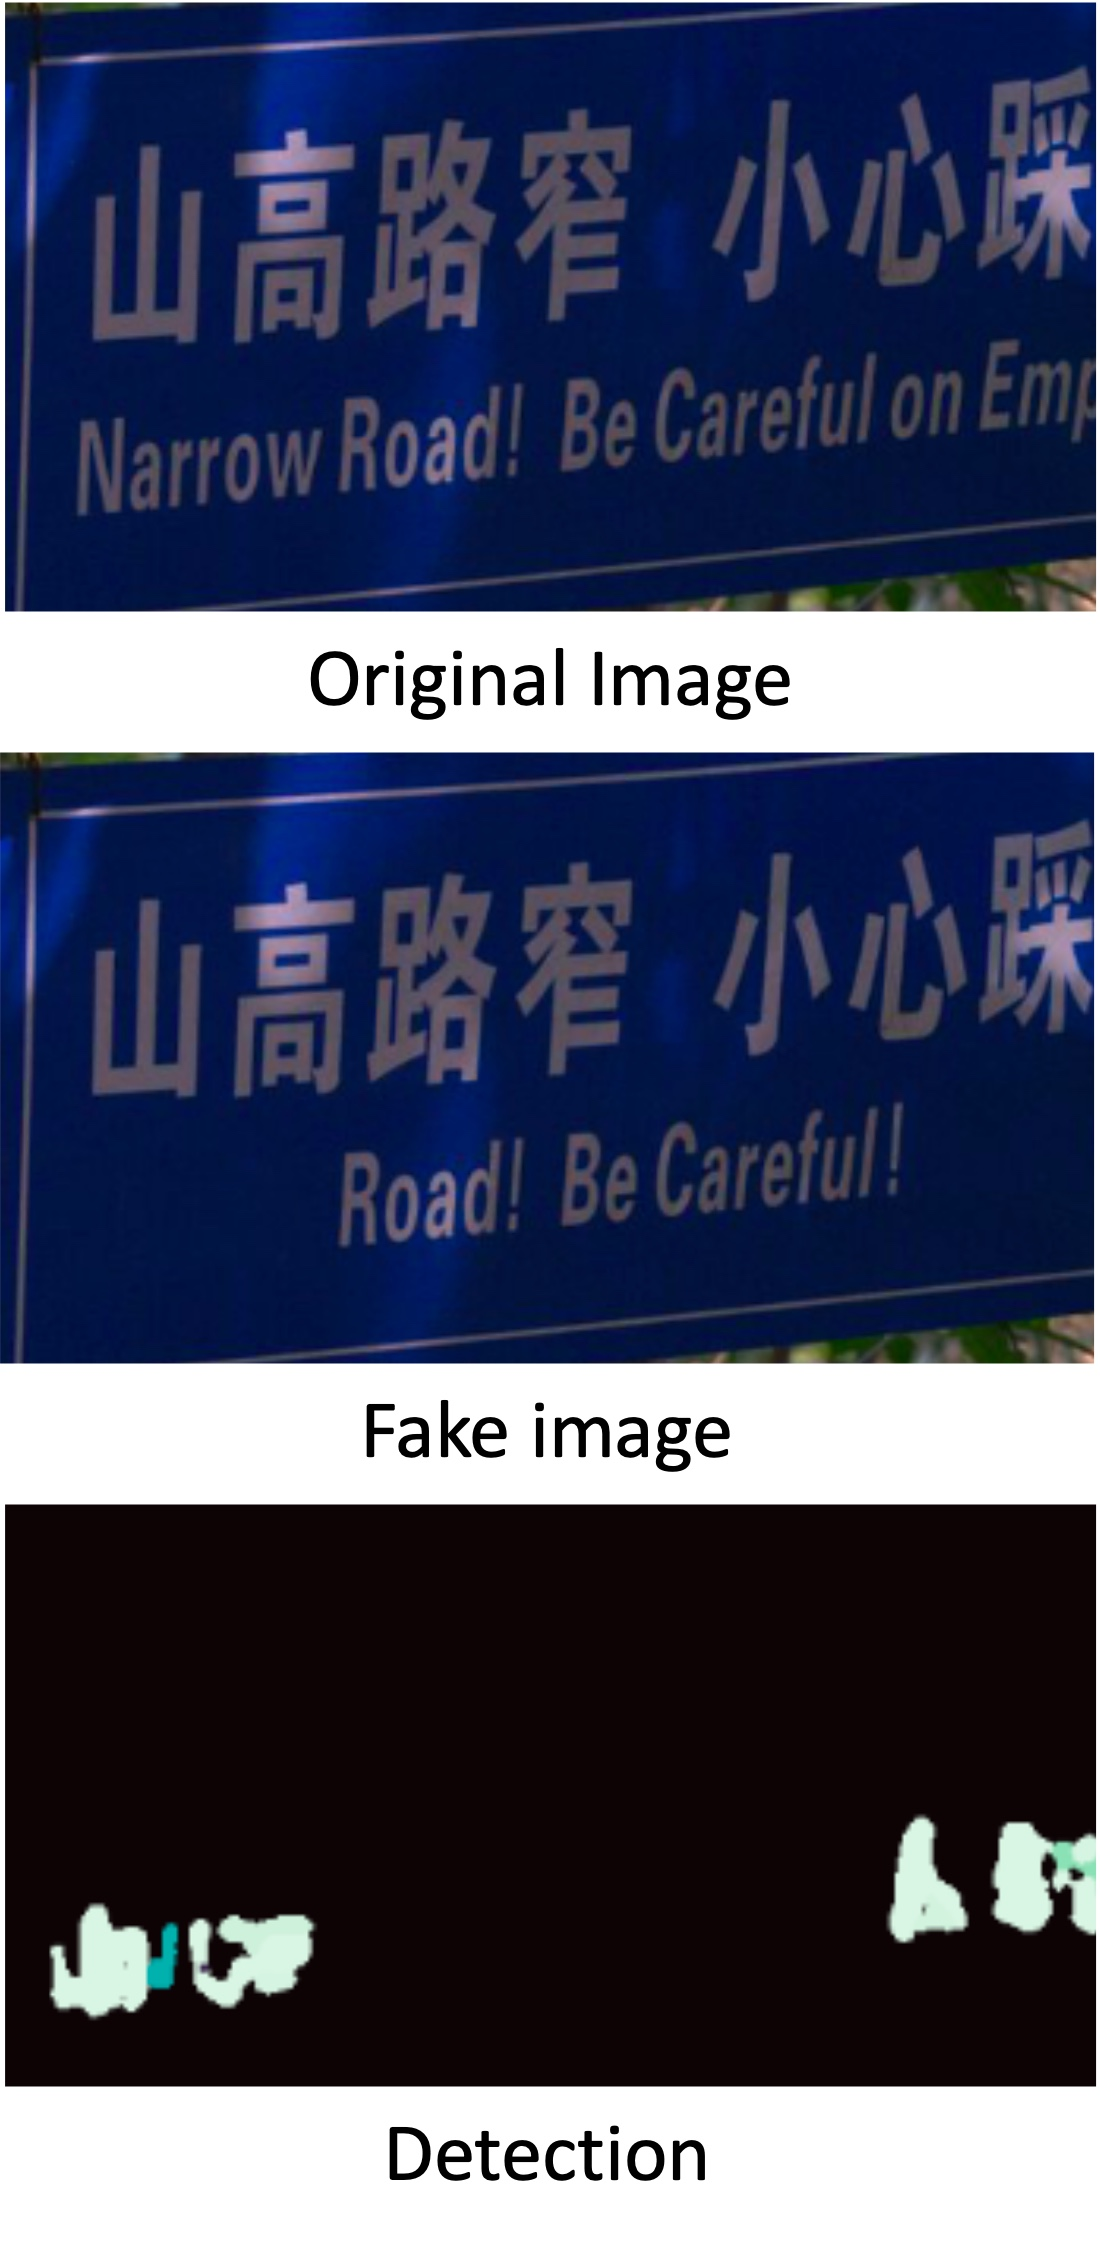
\includegraphics[width=0.7\columnwidth]{figures/Figure 2.jpg}
    \caption{Figure adapted from a figure in \cite{bammey_forgery_2022}: An example of demosaicing-based detection of a fake image. {\normalfont Here, the forgery is not visible at all with the naked eye. The detection is made using the 4Point method, which is a bit different from the one discussed here, yet the general principle remains the same.}}
    \label{fig:example_fake}
\end{figure}

As explained in the paper, the goal of the a contrario framework is to automate the process of deciding whether an image is fake or not, without the need for an expert. Indeed, the fake images that are detected using demosaicing analysis are often not detectable at all with the naked eye. For example, let's take the fake image in figure \ref{fig:example_fake}, and let's refer to the Gestalt theory \cite{von_ehrenfels_uber_1890, morel_detection_2021} to decide what is detectable and what is not. In this image, there is no color discontinuity, no line break or change in the perspective, no shape similarity, nothing that could suggest us that some word have been removed. This difficulty to assess if a image is fake or not makes it crucial to have an automatic pipeline, that does not requires human control and provide a reliable metric to quantify the likelihood of an image to be fake.

\subsection{The a contrario model}

\textit{A contrario detection} is a detection method whose purpose is to automate the decision that, based on observations, decides whether an event has taken place or not, and to quantify the degree of certainty with which these observations allow us to make this decision. This quantification is made with a metric called \textit{number of false alarm} (NFA).

For our task, the a contrario introduced by the authors is the following (cf. section \ref{sec:article_method} and figure \ref{fig:teaser} for a more general presentation of the method):

\begin{itemize}
    \item The image is forged using the 12 configurations (this number of 12 configuration is not the same in the original paper, but the idea remains the same), and we compute the mean reconstruction error for each pixel among the 3 colour channels
    \item Every $2 \times 2$ pixel block votes for the configuration for which the reconstruction error is the lowest
    \item In case of equality, the block votes for randomly for one of the configuration that achieved the minimum. This technical precision is not clearly stated in the original paper, however it is needed for the hypotheses of the a contrario model to be true
\end{itemize}

\subsection{Detecting the global configuration of the image} \label{sec:global_a_contrario}

Thus, in the absence of any demosaicing artefacts, we make the hypothesis that each of the 12 configuration is equally likely. Thus, if we count the votes for each of the 12 configurations, we should roughly count $1/12$ of the total votes for each configuration. 

More precisely, let's quantify the probability that the configuration that gets the most votes gets at least $k$ votes. For this purpose, let's denote by $N_{cfg}$ the number of configuration (here, $12$), $N_{block}$ the number of $2 \times 2$ blocks (roughly the number of pixels divided by 4), and $\text{Binom}_{sf}$ the survival function of the binomial distribution. Then, for each block, there is a probability of $1/12$ to observe a given configuration. Thus, the probability that we observe at least $k$ times this given configuration is:

$$
g(k) = \text{Binom}_{sf}(k, N_{block}, 1/ N_{cfg})
$$

Then, let's take an image and denote by $(X_i)_{1 \le i \le N_{cgf}}$ the number of votes for each configuration. If we take $f(i, k) = N_{cfg} \times g(k)$, using proposition 4 of section 2.5 in \cite{morel_detection_2021}, we obtain that $f$ is a Number of False Alarm (NFA) with respect to the definition 2 section 2.5 of \cite{morel_detection_2021}. Thus, we will call $NFA_{global}(k)$ the following quantity, which can be interpreted as the probability that a image with no demosaicing artefacts lead to a maximal number of votes for a configuration of $k$ or more: 

$$
NFA_{global}(k) = N_{cfg} \times \text{Binom}_{sf}(k, N_{block}, 1/ N_{cfg})
$$

Thus, for a given image, if we observe $k$ votes for the majority vote, and if $NFA_{global}(k)$ is really low (typically, $10^{-6}$ or less), we can say that this image is very unlikely to be free of any demosaicing artefacts, and on the contrary the majority votes is very likely to represent the true configuration used during the caption of the image.

\subsection{Detecting the configuration in small windows of the image} \label{sec:local_a_contrario}

What we just did for the whole image, we can do for a subpart of the image, for example a window of size $W \times W$ blocks. Thus, for each window we have the detection of a configuration. It can happen that the configuration detected for one of the windows is not the same configuration as the one detected for the whole image.

More precisely, we will perform the following series of tests: for each window of size $W \times W$, we count the number of votes for each configuration different from the global configuration of the image. Then, we take the maximum number of votes among these different tests. As before, for each of these tests, the probability of observing a number of votes greater than or equal to $k$ is given by $\text{Binom}_{sf}(k, W^2, 1/ N_{cfg})$. Given that there are $N_{win} \times (N_{cfg} - 1)$ tests, where $N_{win}$ is the number of windows, the NFA associated to the maximum number of votes is:

$$
NFA_{fake}(k) = N_{win} \times (N_{cfg} - 1) \times \text{Binom}_{sf}(k, W^2, 1/ N_{cfg})
$$

Note here that it is not necessary for the windows to be disjointed. Thus, in the case of overlapping windows, each test is not really independent, and the previous formula can therefore be seen as an upper bound on the number of false alarms, and not an exact expression.

Thus, as noted in the original article, this NFA value enables one to keep control, not over the number of blocks that would be falsely detected in authentic images, but more directly over the frequency at which one image would be detected as fake.

Moreover, we note here that our formula is different to the one of the original article: we used $(N_{cfg} - 1)$ instead of $N_{cfg}$ in the number of tests, because we considered that we do count the votes for the configuration that gets the majority in the full image.

\subsection{Doing detection on algorithm, pattern, or diagonal} The same principle can be used, replacing votes for the best approaching configuration, by votes for the best algorithm, pattern, or diagonal. To do this, we take the votes of every $2 \times 2$ block, and give it to the algorithms involved in this configuration, or pattern, or diagonal.

The rest of the reasoning, as well as the NFA formulas presented in the previous sections, remain the same, replacing $N_{cfg}$ either by $3$, $4$, or $2$ depending on whether it is for algorithm, pattern, or diagonal.

\section{Experiments to test the method}

In this section, we will discuss the validity of the hypothesis made on the demosaicing algorithms by the original paper. To do so, we first present two types of experiment we conducted, in order to verify the validity of the NFA computed in section \ref{sec:a_contrario}, which are similar to the ones of the original paper:

\begin{itemize}
    \item First, we conducted experiments on images that were forged \textit{a priori} with various configuration of algorithm and pattern, using various JPEG compression level, to see if the method proposed by the author lead to a correct \textit{a posteriori} detection of the configuration previously used.
    \item Second, we conducted experiments to evaluate the detection of fake images: we took a thousand of images, and for half of them we artificially forged a part of the image with another demosaicing configuration than the rest of the image. Then, we computed the true detection and false detection rates.
\end{itemize}

We also discuss why the NFA provided by the authors seem invalid with our experiments, and what should be done to obtain a robust and trustworthy fake detection method based on demosaicing analysis.

\subsection{Experiments 1: detecting the configuration used during the caption of an image} \label{sec:experiment_1}

To illustrate this experiment, we have prepared a notebook that can be executed as a standalone, and that highlights the important points of this section. This notebook is available \href{https://github.com/DentanJeremie/demosaicing-detection/blob/main/doc/configuration_detection_demonstration.ipynb}{\underline{here}}.

\subsubsection{Experimental protocol} 

First, we wanted to evaluate the effectiveness of the double demosaicing technique proposed by the authors. To do so, we first used a dataset that was also used in the original paper, which is provided by \cite{colom_noise_2023}. This dataset contains 16 high-quality images, which have really low noise since their pixel values were smoothed with a $5 \times 5$ mean pooling. Given the $5 \times 5$ mean pooling of the images, this dataset is claimed to be free of any demosaicing traces by \cite{bammey_demosaicing_2022}. Then we did the following:

\begin{itemize}
    \item For each of the 16 images of the dataset; for each of the 12 configuration (algorithm, pattern) plus an additional configuration where nothing is done; for each of the JPEG compression level 100, 95, 90 (level 100 means no compression); we forged the image. This aim at reproducing and controlling what would be the true configuration used during the caption of the images.
    \item Then, for each of those 702 images, we performed several detections with various NFA thresholds: $t = 1$, $t = 0.01$, $t = 10^{-8}$:
    \begin{itemize}
        \item Detection of the event "no demosaicing is done": for this task, the detection happens when no configuration is detected with NFA smaller than $t$. For this task, there can only be true or false detection (there cannot be no detection).
        \item Detection of the event "demosaicing was done with algorithm A" for A equal to \texttt{bilinear}, \texttt{malvar}, \texttt{menon}: for this task, the detection happens when the algorithm is correctly detected with NFA smaller than $t$; there is no detection if no algorithm is detected with NFA smaller than $t$, and there is a false detection if the wrong algorithm is detected with NFA smaller than $t$.
        \item Detection of the patterns \RGGB, \BGGR, \GRBG, \GBRG, with similar definition as for the algorithm.
        \item Detection of the diagonals \texttt{up} ("0" in the figures) and \texttt{down} ("1" in the figures), with similar definitions as for the algorithm.
    \end{itemize}
\end{itemize}

\subsubsection{Results on the no\_noise\_images dataset}

The result of those simulations using dataset \cite{colom_noise_2023} are presented in figures \ref{fig:config_10-0}, \ref{fig:config_10-2} and \ref{fig:config_10-8}.

\medskip \textbf{Lecture of the figures:} For each of the groups (e.g. "BGGR" or "0"), the left column is without JPEG compression, the middle one is with JPEG95, and the right one with JPEG90. Each column have been normalized to 1, and represent the proportion of true, false, and no detection for this setting (e.g. for group "0", true, false and no detection of diagonal "up" during the detection of the diagonal).

\begin{figure}[p]
    \centering
    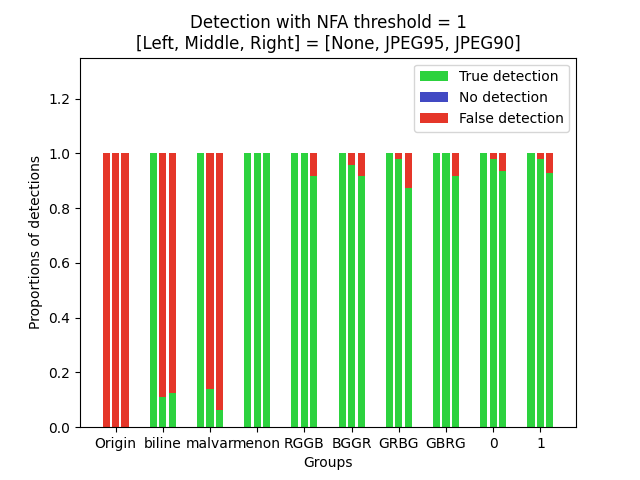
\includegraphics[width=0.87\columnwidth]{figures/config_detection_nfa_1.png}
    \caption{Detection of the configuration used during the caption of the images, NFA = 1, using dataset no\_noise\_images \cite{colom_noise_2023}}
    \label{fig:config_10-0}
\end{figure}

\begin{figure}[p]
    \centering
    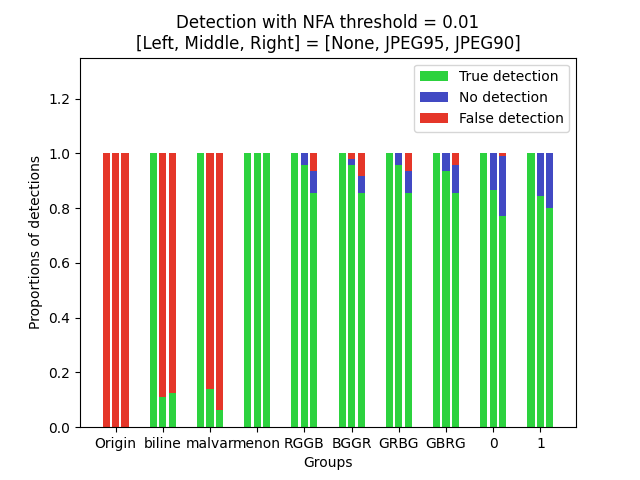
\includegraphics[width=0.87\columnwidth]{figures/config_detection_nfa_0.01.png}
    \caption{Detection of the configuration used during the caption of the images, NFA = 0.01, using dataset no\_noise\_images \cite{colom_noise_2023}}
    \label{fig:config_10-2}
\end{figure}

\begin{figure}[p]
    \centering
    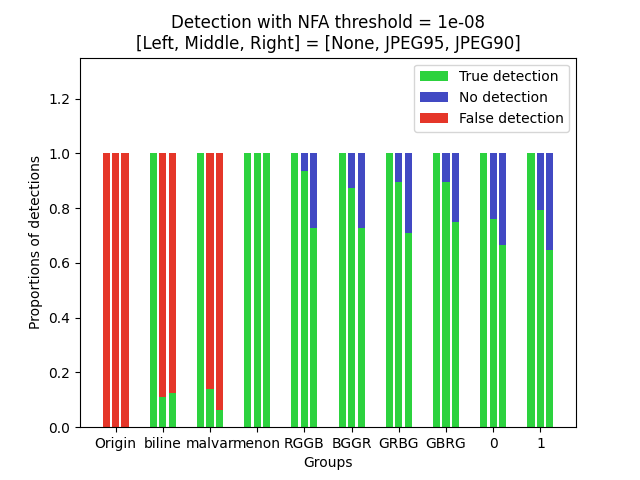
\includegraphics[width=0.87\columnwidth]{figures/config_detection_nfa_1e-08.png}
    \caption{Detection of the configuration used during the caption of the images, NFA = 10-8, using dataset no\_noise\_images \cite{colom_noise_2023}}
    \label{fig:config_10-8}
\end{figure}

\subsubsection{Interpretation} We can make the following observations from  figures \ref{fig:config_10-0}, \ref{fig:config_10-2} and \ref{fig:config_10-8}.

\medskip

First, let's analyse the six groups at the right, i.e. the ones that corresponds to the detection of the pattern or of the diagonal.

\begin{itemize}
    \item As one could expect, we always observe that the performance decrease (i.e. the number of false detection or no detection improves) as the JPEG compression quality decreases. This is visible with red and blue parts of the bars getting bigger when going to the right in a group of three bars. However, as mentioned in the original paper, we observe that the performance remains quite high, and for the detection of the pattern and the diagonal, there is at least 60\% of true detection, even for JPEG90 compression.
    \item Moreover, we observe that when the NFA threshold decreases (i.e. going from figure \ref{fig:config_10-0} to \ref{fig:config_10-2} to \ref{fig:config_10-8}), more and more false detection become no detection, and more and more true detection become no detection. This is exactly what we expect from a NFA: the smaller the threshold is, the more confident we want to be on our detections, which removes some false detection, at the cost of loosing some true ones.
    \item More precisely, the number of false detection is coherent with the theoretical values of the NFA. Indeed, as shown in table \ref{tab:false_detection}, the proportion of false detection is equal or inferior to the NFA. For example, with NFA threshold set at $10^{-2}$, we observe precisely 1\% of false alarm. And with 1152 tests, we observe no false detection with threshold $10^{-8}$, as expected.
\end{itemize}

Thus, the theory developed in section \ref{sec:a_contrario} seems coherent with the experiments we conducted for pattern and diagonal detection (the six groups at the right).

\begin{table}[!h]
\centering
\begin{tabular}{|
>{\columncolor[HTML]{EFEFEF}}c |c|c|}
\hline
\textbf{NFA threshold} & \cellcolor[HTML]{EFEFEF}\textbf{\begin{tabular}[c]{@{}c@{}}False detection\\ (1152 tests)\end{tabular}} & \cellcolor[HTML]{EFEFEF}\textbf{Proportion} \\ \hline
$10^{0}$ & 37 & $3.2 \times 10^{-2}$ \\ \hline
$10^{-2}$ & 12 & $1.04 \times 10^{-2}$ \\ \hline
$10^{-8}$ & 0 & 0 \\ \hline
\end{tabular}
\bigskip
\caption{Evolution of the proportion of false detection when decreasing the NFA threshold for the detection. {\normalfont The 1152 tests correspond only to the detection of the pattern or the diagonal (6 right columns on figures \ref{fig:config_10-0}, \ref{fig:config_10-2} and \ref{fig:config_10-8}). These experiments confirm that the NFA theoretically computed in section \ref{sec:a_contrario} are indeed upper bounds on the expectations of the number of false alarms. This table is adapted from a more complete table available in the \texttt{output} directory of the repository \href{https://github.com/DentanJeremie/demosaicing-detection}{\underline{here}}.}}
\label{tab:false_detection}
\end{table}

However, what we observe with the four groups at the left (i.e. detection of the absence of demosaicing or detection of the algorithm) is totally incoherent with the theory developed in section \ref{sec:a_contrario}:

\begin{itemize}
    \item The number of false detection is much greater than the NFA: there is a total of 624 tests for those four columns, and a least 276 false detection (about 44\%) for every NFA threshold, even $10^{-8}$!
    \item For every image that was not demosaiced, no matter the JPEG compression or the NFA threshold, there is always a false detection of a demosaicing configuration. 
\end{itemize}

There are several ways to interpret this:

\begin{itemize}
    \item First, to explain that a demosaicing is always detected, even when nothing is done, we can make the hypothesis that the images of the dataset \cite{colom_noise_2023} are not free of any demosaicing traces. However, this hypothesis does not stand, for several reasons:
    \begin{itemize}
        \item First, those images are obtained after a $5 \times 5$ mean pooling. Given that the CFA grid is $2$-periodic, every pixel value of the final images comes from many true and interpolated pixel values, making it really unlikely that demosaicing artefacts remain after the pooling.
        \item Second, we have conducted the same experiments with images that are for sure free of any demosaicing artefacts because they are computer-generated (cf. section \ref{sec:exp_dall_e}), so no CFA grid was never preset during the creation of the image. And with those computer generated images, the observed the same rate of false detection.
    \end{itemize}
    \item Second, we can make the hypothesis that some demosaicing algorithms are intrinsically better than others in some situation, leading to their false detection. This hypothesis contradicts the a-contrario model, because this model makes the hypothesis that in the absence of demosaicing artefacts, every configuration is equally likely to get the vote of a $2 \times 2$ block. This could explain all our observation of abnormally high false detection rate:
    \begin{itemize}
        \item In the absence of any demosaicing artefacts (first group at the left), given that some algorithms are intrinsically better than others, many blocks of $2 \times 2$ vote for them, leading to their false detection with very low NFA value.
        \item For any of the three groups \texttt{bilinear}, \texttt{malvar}, \texttt{menon}, there is 100\% of true detection without JPEG compression, but the problem of false detection appears with the JPEG compression. This can be explained with the hypothesis we just made: when the image is compressed, the demosaicing artefacts are less visible, so the true algorithm is less favored for the votes. Thus, a lot of $2 \times 2$ blocks vote for the most performant algorithm rather than one that left some hardly-detectable demosaicing artefacts.
        \item With our observation, it is likely that algorithm \texttt{menon} is more performant than the other, because it is not really concerned by this apparition of false detection when compression increases.
    \end{itemize}
\end{itemize}

\subsubsection{Results on the dall\_e\_images dataset} \label{sec:exp_dall_e}

As said above, to refute the hypothesis that the images of the no\_noise\_dataset \cite{colom_noise_2023} contain some demosaicing artefact, we performed the same experience on images that are truly free of any demosaicing artefacts since they are computer-generated. To do so, we generated 18 images using DALL-E software \cite{ramesh_hierarchical_2022}. For more simplicity, the results are not presented here, however they are available in the \texttt{output} directory of the repository \href{https://github.com/DentanJeremie/demosaicing-detection}{\underline{here}}.

The results of those experiments are clear: we observe the same type of result as with the no\_noise\_images dataset, refuting this hypothesis.

\subsubsection{Hardware and computation time} For this experiment, we used an Intel Xeon W-1290P 3.70GHz. To process the 16 images of dataset \cite{colom_noise_2023} using a single thread, this experiment took about 8min, i.e. about 30s per image for all the tests (the images have shape $704\times469$).

\subsubsection{Conclusion on experiment 1} 

The method described by the original article seems to work really well for the detection of the demosaicing patter, even when the images are compressed. For those detections, the numbers of false detection are coherent with the NFA we computed theoretically, which are thus empirically validated.

However, for the detection of the demosaicing algorithm or the detection of the absence of demosaicing, the method lead to a really high proportion of false detection, making it unreliable. To explain those false detections, we retain our second hypothesis, that explains all our observations : \textbf{some demosaicing algorithms are intrinsically better than other,} which contradicts the uniform distribution of the a contrario model, resulting in much higher false detection that what we expected based on our NFA computations. This issue has no consequence on the detection of the pattern and of the diagonal, but misleads both the detection of the absence of demosaicing, and the detection of a given demosaicing algorithms. Obviously, this will have consequences on the performance of the forgery detection pipeline.

\subsection{Experiment 2: detecting if an image is fake or not} \label{sec:experiment_2}

To illustrate this experiment, we have prepared a notebook that can be executed as a standalone, and that highlights the important points of this section. This notebook is available \href{https://github.com/DentanJeremie/demosaicing-detection/blob/main/doc/forgery_detection_demonstration.ipynb}{\underline{here}}.

\subsubsection{Experimental protocol} 

After evaluating the performance of demosaicing detection, we conducted a second group of experiments with the objective of evaluating the detection of fake images based on demosaicing detection.

Of course, the problems described above that affect demosaicing detection, especially in the absence of demosaicing artifacts, are still present and have repercussions on the detection of fakes.

We conducted the following experiments:

\begin{itemize}
    \item We have generated 3 times 1000 random fake images, one for every compression factor equals to $100$, $95$, or $90$, using the following method:
    \begin{itemize}
        \item We randomly sample an integer between 0 and 17, and take the image with the corresponding index in the dataset
        \item We randomly sample an integer between 0 and 11, and forge the full image with the corresponding (algorithm, pattern) configuration
        \item We randomly sample the position of a $200 \times 200$ window where we will imitate a fake 
        \item We randomly sample an integer between 0 and 2, and with this integer we select one of the 3 pattern that was not used for the full image. Then, we forge the windows with this pattern, and with the same algorithm as the one used for the full image. The fact that we only change the pattern comes from the difficulty to detect the algorithm, as discussed for our first experiment in section \ref{sec:experiment_1}.
        \item We apply the JPEG compression at the end if needed
    \end{itemize}
    \item We have generated 3 times 500 random non-fake image, one for every compression factor equals to $100$, $95$, or $90$, using the following method. With this method, the images are not fake, however they are forged to imitate some natural demosaicing artefacts that would be left by a camera.
    \begin{itemize}
        \item We randomly sample an integer between 0 and 17, and take the image with the corresponding index in the dataset
        \item We randomly sample an integer between 0 and 11, and forge the full image with the corresponding (algorithm, pattern) configuration
        \item We apply the JPEG compression at the end if needed
    \end{itemize}
\end{itemize}

Then for every JPEG compression level, we deploy the fake image detection pipeline presented in section \ref{sec:a_contrario}, and count the true detection, false detection, and no detection. More precisely:

\begin{itemize}
    \item For fake image, there is either a true detection or a no detection
    \item For an non-fake image, there is either a false detection or a true detection
\end{itemize}

\subsubsection{Results of the simulation}

The results of those experiments are presented below in figures \ref{fig:fake_10-0}, \ref{fig:fake_10-2} and \ref{fig:fake_10-8}.

\medskip \textbf{Lecture of the figures:} For each of the groups \texttt{fake} (called \texttt{forge} here due to an inconsistency in the naming) and \texttt{non-fake} (called \texttt{unforged} here due to an inconsistency in the naming), the left column is without JPEG compression, the middle one is with JPEG95, and the right one with JPEG90. Each column have been normalized to 1, and represents the proportion of true, false, and no detection for this setting.

\begin{figure}[p]
    \centering
    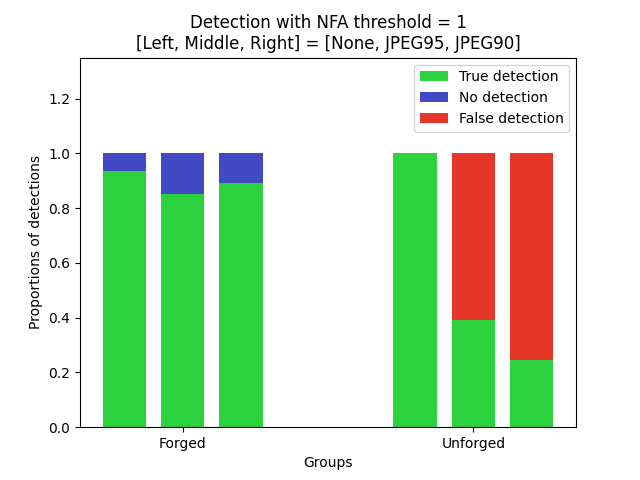
\includegraphics[width=0.93\columnwidth]{figures/forgery_detection_nfa_1.png}
    \caption{Detecting if there is a fake area in the image, NFA = 1, using dataset no\_noise\_images \cite{colom_noise_2023}}
    \label{fig:fake_10-0}
\end{figure}

\begin{figure}[p]
    \centering
    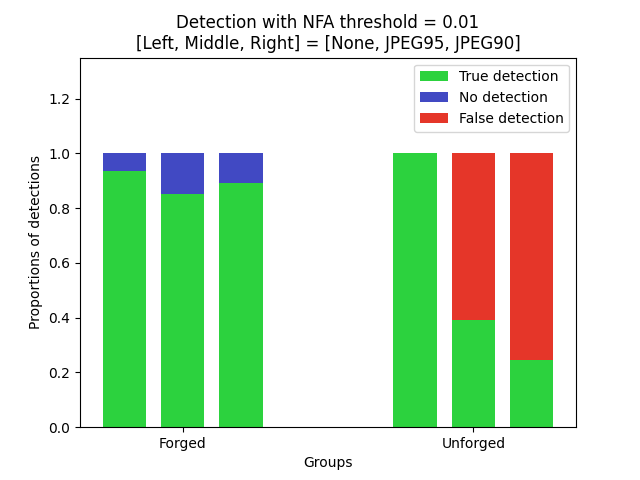
\includegraphics[width=0.93\columnwidth]{figures/forgery_detection_nfa_0.01.png}
    \caption{Detecting if there is a fake area in the image, NFA = 1, using dataset no\_noise\_images \cite{colom_noise_2023}}
    \label{fig:fake_10-2}
\end{figure}

\begin{figure}[p]
    \centering
    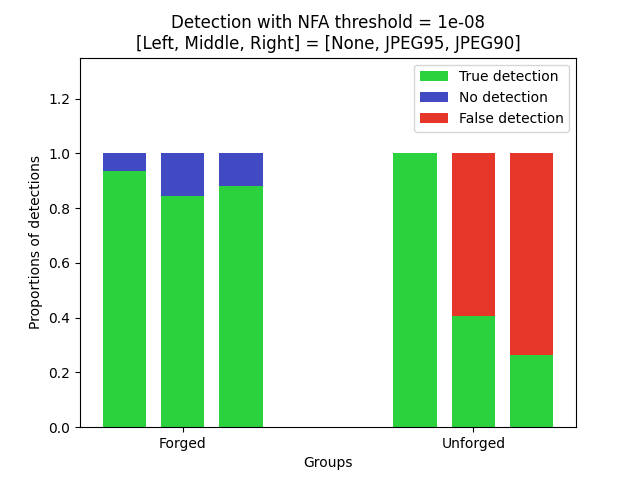
\includegraphics[width=0.93\columnwidth]{figures/forgery_detection_nfa_1e-08.png}
    \caption{Detecting if there is a fake area in the image, NFA = 1, using dataset no\_noise\_images \cite{colom_noise_2023}}
    \label{fig:fake_10-8}
\end{figure}

\subsubsection{Interpretation of the results} We can make the following observations from  figures \ref{fig:fake_10-0}, \ref{fig:fake_10-2} and \ref{fig:fake_10-8}:

\begin{itemize}
    \item The method developed by the original article seems to be quite effective in detecting fake images (in more than 80\% of cases, even 90\% for uncompressed images). Moreover, in the absence of compression, the method does not make any false detection on the non-fake images.
    \item For the fake images, we can see that the number of non-detections is greater in the presence of compression than in its absence, as we would expect. However, it is surprising that this number is higher in JPEG95 than in JPEG90.
    \item The number of false detections of non-fake images is abnormally high as soon as the images are compressed, even in good quality. This is quite surprising, especially since the detection here only concerns the demosaicing pattern, which was however relatively well detected in JPEG95 and JPEG90 (cf. section \ref{sec:experiment_1}).
\end{itemize}

One hypothesis that could explain this abnormally high number of false detections is that the colors of some textures are better interpolated with some patterns than with others. This would lead some regions of the image to be more likely to vote for patterns that do not have the majority vote for the whole image. However, we were not able to conduct an experiment to test this hypothesis, and we leave this to future work.

On the other hand, it is true that our experiments focus on images that are not genuine fakes generated in order to distort an image. It is therefore possible that this abnormally high number of false detections differs on real images. However, our fake image generation process is a priori easier to detect, because we directly and artificially introduced an inconsistency in the demosaicing artefacts. We therefore leave to future work the task of evaluating this method on a dataset of genuine fake images.

\subsubsection{Hardware and computation time} For this experiment, we used an Intel Xeon W-1290P 3.70GHz. The generation of $3\times1000$ fake images with a single thread took about 227s (3min47, about 75ms per image). The generation of $3\times1000$ non-fake images with a single thread took about 213s (3min33, about 71ms per image). Then, still with a single process, it took about 5058s to do the detection on the 6000 images, i.e. about 843ms per image (the images have shape $704\times469$).

\subsubsection{Conclusion on experiment 2}

This experiment showed that the forgery detection method proposed by the paper is relatively efficient to detect fake images, even compressed. However, the abnormally high number of false detections makes the detections from this method unreliable. Our simulations therefore suggest that this method needs to be reworked before it can be qualified for use on real data.

\section{Conclusion}

In conclusion, our experiments have shown that the method described in the article under review is promising, but that some aspects need to be improved to allow reliable and industrially usable detections. 

First, the first experiment of our study focused on the detection of the demosaicing algorithm and pattern used during the caption of images. We observed that the proposed method worked very well for the detection of the demosaicing pattern, even in the presence of compression; and that it also worked well for the detection of the demosaicing algorithm, in the absence of compression. However, this experiment also showed that the better performances of some demosaicing algorithms can lead to an abnormally high number of false demosaicing detections with respect to the theoretically calculated NFA, when the images are compressed. Thus, in order to obtain a reliable method, it is necessary to validate the hypotheses of the a contrario model, which is not done in the article. This validation could take the form of an evaluation on a large set of images free of demosaicing artefacts (e.g. computer generated images or images obtained after a mean pooling), and for which the different algorithms must have similar performances.

Then, the second experiment of our study focused on the detection of fake images, i.e. images for which a distortion has been artificially added in the demosaicing pattern. We observed good performance in detecting fake images, even in the presence of compression, and no false detection in the absence of compression. However, the number of false detections in the absence of compression makes this method too unreliable until it is improved.

%%
%% The next two lines define the bibliography style to be used, and
%% the bibliography file.
\bibliographystyle{ACM-Reference-Format}
\bibliography{references}


\end{document}
\endinput
%%
%% End of file `sample-sigconf.tex'.
